%\addcontentsline{toc}{part}{Anhang}
%\markright{Anhang}


%\includepdf[pages=2, scale=1, offset= 0cm 0cm, clip, trim= 0cm 0cm 0cm 0cm, pagecommand={\thispagestyle{empty}\chapter{<chapter>}]{<Dateiname>.pdf}
%trim: left bottom right top

\chapter{Herleitung der Wellengleichungen ebener, harmonischer Wellen}\label{Anhang:Herleitung_Wellengleichung}

Ausgangspunkt für die folgende Herleitung nach~\cite{EM_Schirmung} sind die Maxwell'schen Gleichungen~\cite{Maxwell} für ein isotropes und homogenes Ausbreitungsmedium ohne Raumladungen, sodass sich reine Wirbelfelder ausbilden können. Außerdem sei Linearität und Zeitinvarianz des Mediums vorausgesetzt:

\begin{subequations}
    \begin{align}
        \text{rot} \; \vec E &= - \frac{\partial \vec B}{\partial t} = - \mu \frac{\partial  \vec H}{\partial t} \\
        \text{rot} \; \vec H &= \vec J + \frac{\partial  \vec D}{\partial t} = \sigma \vec E + \varepsilon \frac{\partial  \vec E}{\partial t}
    \end{align}
\end{subequations}

%J = elektrische Stromdichte
Mit der Vektoridentität $\text{rot} \; (\text{rot} \; \vec A) = \text{grad} \; (\text{div} \; \vec A) - \Delta \; \vec A$ \cite{Merzinger} können die Gleichungen entkoppelt werden. Setzt man Quellenfreiheit voraus, d.h. sind nur Wirbelfelder vorhanden, lässt sich sogar schreiben:

\begin{equation}
    \text{rot} \; (\text{rot} \; \vec A) = - \Delta \; \vec A
\end{equation}

Damit lassen sich nach der Rotationsbildung 

\begin{subequations}
    \begin{align}
        \text{rot} \; (\text{rot} \; \vec E) &= - \text{rot} \; (\mu \frac{\partial  \vec H}{\partial t}) = - \mu \left(\sigma \frac{\partial  \vec E}{\partial t} + \varepsilon \frac{\partial ^2\vec E}{\partial t^2}\right) \\
        \text{rot} \; (\text{rot} \; \vec H) &= \text{rot} \; (\sigma \vec E + \varepsilon \frac{\partial  \vec E}{\partial t}) = - \sigma \mu \frac{\partial \vec H}{\partial t} - \varepsilon \mu \frac{\partial ^2 \vec H}{\partial t^2} \; ,
    \end{align}
\end{subequations}

bei der entsprechend der vorausgesetzten Linearität die dargestellten Vereinfachungen beim Einsetzen der Vektoridentität vorgenommen wurde, die sogenannten Telegraphengleichungen mit der Wellenausbreitungsgeschwindigkeit $v = \frac{1}{\sqrt{\varepsilon \mu}}$ bilden~\cite{EM_Schirmung}:

\begin{subequations}
    \label{eq:A_Telegraphengleichungen}
    \begin{align}
        \Delta \; \vec E(\vec x,t) = \varepsilon \mu \frac{\partial ^2 \vec E}{\partial t^2} + \sigma \varepsilon \frac{\partial  \vec E}{\partial t}  = \frac{1}{v^2} \frac{\partial ^2 \vec E}{\partial t^2} + \sigma \varepsilon \frac{\partial  \vec E}{\partial t} \label{subeq:A_Telegraphengleichungen1}\\
        \Delta \; \vec H(\vec x,t) = \varepsilon \mu \frac{\partial ^2 \vec H}{\partial t^2} + \sigma \varepsilon \frac{\partial  \vec H}{\partial t} = \frac{1}{v^2} \frac{\partial ^2 \vec H}{\partial t^2} + \sigma \varepsilon \frac{\partial  \vec H}{\partial t}  \label{subeq:A_Telegraphengleichungen2}
    \end{align}
\end{subequations}

Im Folgenden lassen sich zwei Fälle unterscheiden. Dies ist zum einen die Ausbreitung in einem nichtleitenden Medium ($\sigma = 0$), wie zum Beispiel Vakuum, und zum anderen der Fall $\sigma \neq 0$. 

\subsubsection{Fall~\uproman{1} ($\sigma = 0$)}

Hier vereinfachen sich die \Gleichungen~\eqref{eq:A_Telegraphengleichungen} zu hyperbolischen Differentialgleichungen zweiter Ordnung. Im homogenen Fall, in dem die Welle nur durch das Medium geleitet und nicht von ihm erzeugt wird, und für drei Raumdimensionen haben die Gleichungen die Form

\begin{equation}
     \frac{1}{v^2}\frac{\partial ^2 u}{\partial t^2} - \Delta u = \frac{1}{v^2}\frac{\partial ^2 u}{\partial t^2} -  \mathlarger{\mathlarger{\sum}}_{i=1}^3 \frac{\partial^2 u}{\partial x_i^2} = 0   \; \text{.}
\end{equation}

Für die Betrachtung ebener Wellen ist nur eine Raumrichtung relevant. Weiterhin lassen sich allgemeine Lösungen der dreidimensionalen Wellengleichung als Linearkombination ebener Wellen bilden. Hier wird als Ausbreitungsrichtung die Komponente $x_1 = x$ des Koordinatenvektors $\vec x$ genutzt. Man erhält

\begin{equation}
    \frac{1}{v^2}\frac{\partial^2 u}{\partial t^2} - \frac{\partial^2 u}{\partial x^2} = 0 \; ,
\end{equation}

was sich für eine mehrfach stetig differenzierbare Funktion $u$ mit dem Satz von Schwarz\footnote{Satz von Schwarz: Für eine $k$-mal stetig partiell differenzierbare Funktion $f : D \subset \mathbb{R}^m \to \mathbb{R}$ mit $m$ Variablen gilt, dass diese ebenfalls $k$-mal stetig total differenzierbar ist und die partiellen Ableitungen jeder Ordnung $j \leq k$ unabhängig von der Reihenfolge der Differentiationen sind~\cite{Vorlesung_Ingenieursmathematik}} zu

\begin{equation}
    \left(\frac{1}{v} \frac{\partial u}{\partial t} - \frac{\partial u}{\partial x}\right) \cdot \left(\frac{1}{v} \frac{\partial u}{\partial t} + \frac{\partial u}{\partial x}\right) = 0
\end{equation}

umstellen lässt. \par
Damit wird die Struktur der Lösung für die allgemeine Funktion $u(x,t)$ 

\begin{equation}
    u(x,t) = f(x+vt) + g(x-vt)
\end{equation}

ersichtlich~\cite{Methoden_physikalischer_Mathematik_Band_2}. $f$ und $g$ sind zwei beliebige, zweifach stetig differenzierbare Funktionen, die jeweils einen in positiver x-Richtung und einen in negativer x-Richtung ausbreitenden Wellenanteil beschreiben. Für die weitere Betrachtung ist eine Beschränkung auf eine einseitig ausbreitende Welle (vgl.~\Abb \ref{subfig:2_Hertzscher_Dipol_B}) ausreichend, da sich dafür die Phänomene wie Dämpfung und Reflektion in gleichem Maße beschreiben lassen~\cite{EM_Schirmung}. Die Integrationskonstante kann ebenfalls vernachlässigt werden, die sie ein Gleichfeld beschreibt, welches für die Betrachtung von Welleneigenschaften nicht von Bedeutung ist~\cite{EM_Schirmung}. Somit lauten die erhaltenen Lösungen der Wellengleichung

\begin{subequations}
    \begin{align}
        \vec E = \vec E(x-vt) \\
        \vec H = \vec H(x-vt)
    \end{align}
\end{subequations}

für sich ungedämpft und unverzerrt ausbreitende Wellen. Wie bereits erwähnt können $\vec E$ und $\vec H$ dabei beliebige, zweifach stetig differenzierbare Funktionen sein. Im Fall der harmonischen Anregung mit der Frequenz $f$ bzw. der Kreisfrequenz $\omega = 2\pi f$ ergeben sich gut zu beschreibende Zeitverläufe, mit deren Grundlage sich mittels der Fourier-Transformation in linearen Ausbreitungsmedien beliebige Zeitverläufe beschreiben lassen. \par
Für die Darstellung ist es zweckmäßig, die Wellenzahl $k = 2\pi / \lambda = \omega \sqrt{\varepsilon \mu}$ einzuführen~\cite{EM_Schirmung}. Damit gilt unter Verwendung der Euler'schen Form $e^{jx} = \cos{x} + j \sin{x}$~\cite{Merzinger}:
\begin{subequations}
    \begin{align}
        \vec E(x,t) &= E_0 \cdot e^{j (\omega t - k x)} \vec e_y \\
        \vec H(x,t) &= H_0 \cdot e^{j (\omega t - k x)} \vec e_z
    \end{align}
    \label{eq:A_Wellengleichungen}
\end{subequations}

für die Feldstärkevektoren in y- bzw. z-Richtung. Im \Abschnitt \ref{cha:2_sub_Feldverlauf_in_Umgebung_eines_Dipols} wurde bereits erläutert, dass in großem Abstand von der Quelle das elektrische und magnetische Feld jeweils nur noch eine Raumkomponente aufweisen, die außerdem nicht entlang der Ausbreitungsrichtung der Welle ausgerichtet ist.


\subsubsection{Fall~\uproman{2} ($\sigma \neq 0$)}

Unter Berücksichtigung der Leitfähigkeit $\sigma$ des Ausbreitungsmediums tritt bei der Ausbreitung der Welle im Raum eine Dämpfung auf. Für die Betrachtung werden wieder die \Gleichungen \eqref{eq:A_Telegraphengleichungen} herangezogen. Wie im Fall~\uproman{1} soll sich die Beschreibung hier auf die Ausbreitung der Welle in einer Raumrichtung mit den Komponenten $E_y$ und $H_z$ orthogonal dazu und auf eine harmonische Anregung beschränken. Unter dieser Voraussetzung lassen sich die \Gleichungen \eqref{eq:A_Telegraphengleichungen} folgendermaßen schreiben~\cite{EM_Schirmung}:

\begin{subequations}
    \begin{align}
        \frac{\partial^2 E_y}{\partial x^2} e^{j\omega t} &= \sigma \mu \omega j E_y e^{j \omega t} + \varepsilon \mu (- \omega)^2 E_y e^{j \omega t} \\
        \frac{\partial^2 H_z}{\partial x^2} e^{j\omega t} &= \sigma \mu \omega j H_z e^{j \omega t} + \varepsilon \mu (- \omega)^2 H_z e^{j \omega t}
    \end{align}
\end{subequations}

Für die bessere Darstellung der Lösung kann auch hier die Wellenzahl $k$ 

\begin{equation}
    k = \sqrt{\varepsilon \mu \omega^2 - j \omega \sigma \mu}
\end{equation}

eingeführt werden, die jetzt allerdings komplex ist. \par
In gleicher Weise wie im Fall~\uproman{1} erhält man die Lösung der Diffenrentialgleichung~\cite{Methoden_physikalischer_Mathematik_Band_2} mit der komplexen Wellenzahl $k$:

\begin{subequations}
    \begin{align}
        \vec E(x,t) &= E_0 \cdot e^{j (\omega t - k x)} \vec e_y \\
        \vec H(x,t) &= H_0 \cdot e^{j (\omega t - k x)} \vec e_z \nonumber \\
                    &= \frac{E_0}{Z} \cdot e^{j (\omega t - k x)} \vec e_y
    \end{align}
    \label{eq:A_Wellengleichungen_mit_Leitfaehigkeit}
\end{subequations}

Der Feldwellenwiderstand $Z$ (vgl.~\Abschnitt \ref{cha:2_sub_Feldverlauf_in_Umgebung_eines_Dipols}) ist das Verhältnis der Feldvektoren

\begin{equation}
    Z = \frac{\vec E}{\vec H} = \frac{\mu \omega}{k} = \sqrt{\frac{j \omega \mu}{\sigma + j \omega \varepsilon}}
\end{equation}

und in diesem Fall ebenfalls komplex.






\RedeclareSectionCommand[beforeskip=-\topskip]{chapter}  %weniger Whitesapce über der Kapitelüberschrift


\includepdf[pages = 1, scale = 0.8, offset = 0cm -2cm, pagecommand={\thispagestyle{empty}\chapter{Nomogramm zur Bestimmung der Reflektionsdämpfung ebener Wellen}\label{Anhang:Nomogramm_Reflektionsdaempfung}
Das nachfolgende Nomogramm dient der graphischen Ermittlung der Reflektionsdämpfung ebener Wellen an ausgewählten Materialien\footnote{Richtwerte für Materialkennwerte nach~\cite{Simplified_shielding}} und wurde nach der folgenden Rechenvorschrift~\cite{Simplified_shielding} gebildet:

\begin{equation}
    R_w \; \left[\text{dB}\right] \approx 168 + 10 \cdot \log_{10}\left(\frac{\sigma_r}{\mu \cdot f}\right)
\end{equation}}]{Anhang/Nomogramm_Reflektionsdaempfung.pdf}


\includepdf[pages = 1, scale = 0.8, offset = 0cm -2cm, pagecommand={\thispagestyle{empty}\chapter{Nomogramm zur Bestimmung der Absorptionsverluste in Schirmen}\label{Anhang:Nomogramm_Absorptionsverlust}

Das nachfolgendene Nomogramm dient der graphischen Ermittlung der Absorptionsverluste in Schirmmaterialien\footnote{Richtwerte für Materialkennwerte nach~\cite{Simplified_shielding}} und wurde nach der folgenden Rechenvorschrift~\cite{Simplified_shielding} gebildet:

\begin{equation}
    A_w \; \left[\text{dB}\right] \approx 131,5 \cdot t \cdot \sqrt{\sigma_r \cdot \mu \cdot f}
\end{equation}}]{Anhang/Nomogramm_Absorptionsverlust.pdf}


\RedeclareSectionCommand{chapter}    

\thispagestyle{fancy}



\chapter{Anforderungsliste}\label{A:Anforderungsliste}


\centering
%\rmfamily

\begin{longtable}{p{1cm}p{1cm}p{13.2cm}} 

    \caption{Anforderungsliste des Fernfeldmesstandes}\\[1.2\normalbaselineskip]
    \toprule 
    \textbf{ID}&\textbf{F/W}&\textbf{Anforderung}\\
    \toprule 
    \endfirsthead 
    \caption[]{Anforderungsliste des Fernfeldmessstandes \emph{(Fortsetzung)}}\\[1.2\normalbaselineskip] 
    \toprule 
    \textbf{ID}&\textbf{F/W}&\textbf{Anforderung}\\
    \toprule 
    \endhead 
    \midrule\nopagebreak 
    \multicolumn{3}{c}{\dots}
    \endfoot 
    \bottomrule 
    \endlastfoot

    \multicolumn{3}{l}{\textbf{Geometrie}} \\
    \midrule
    \theKat.\theID  & F     & Maße:               \newline
                                \noindent\hspace*{4mm} - Länge: $\approx$ \SI{2000}{\milli\meter} (vgl. Abschätzungen in \Kapitel\ref{cha:3}) \newline
                                \noindent\hspace*{4mm} - Breite: $\approx$ \SI{1500}{\milli\meter} \newline
                                \noindent\hspace*{4mm} - Höhe:~~$\approx$ \SI{1500}{\milli\meter}        \stepcounter{ID} \\ 
    \theKat.\theID  & F     & Maße der Prüfkörper (Folien und Schäume): \newline
                                \noindent\hspace*{4mm} - \SI{120}{\milli\meter}$\; \times \;$\SI{120}{\milli\meter}; Messausschnitt: \SI{100}{\milli\meter}$\; \times \;$\SI{100}{\milli\meter} \newline
                                \noindent\hspace*{4mm} - Folienstärke: $\leq$ \SI{2}{\milli\meter} \newline
                                \noindent\hspace*{4mm} - Schaumstärke: $\leq$ \SI{12}{\milli\meter} \stepcounter{ID} \\
    \theKat.\theID  & W     & Test unterschiedlicher Prüfkörperstärken mit gleicher Halterung \stepcounter{ID} \\
    \midrule
    \multicolumn{3}{l}{\textbf{Kinematik}} \stepcounter{Kat} \setcounter{ID}{1} \\ 
    \midrule
    \theKat.\theID  & F     & Positionierung der Prüfkörper im Versuchsstand    \newline
                                \noindent\hspace*{4mm} - Positionsabweichung in Höhe und Tiefe des Versuchsstandes: \SI{\pm1}{\centi\meter}  \newline
                                \noindent\hspace*{4mm} - Positionsabweichung zwischen Antennen: \SI{\pm1}{\centi\meter}  \stepcounter{ID} \\ 
    \theKat.\theID  & F     & Positionierung der Antennen im Versuchsstand \newline
                                \noindent\hspace*{4mm} - Positionsabweichung in Höhe und Tiefe des Versuchsstandes: \SI{\pm1}{\centi\meter} \stepcounter{ID} \\
    \theKat.\theID  & F     & Ebenheit des Reflektors \newline 
                                \noindent\hspace*{4mm} - Winkelabweichung des Reflektors orthogonal zur Senderichtung: \SI{2}{\degree} \stepcounter{ID} \\
    \theKat.\theID  & W     & Versuchsstand rollbar für bessere Umpositionierung im Labor \stepcounter{ID} \\

    \midrule
    \multicolumn{3}{l}{\textbf{Festigkeit}} \stepcounter{Kat} \setcounter{ID}{1} \\ 
    \midrule

    \theKat.\theID  & F     & Keine plastische Verformung der gewichtstragenden Bauteile    \stepcounter{ID} \\
    \theKat.\theID  & W     & Geringe elastische Verformung bei Betreten des Versuchsstandes für Montage und Anpassungen \stepcounter{ID} \\
    \theKat.\theID  & F     & Geringe elastische Verformung der Durchführungsverschlüssse (Türblätter) bei Schließen gegen verwendete HF-Dichtungen \stepcounter{ID} \\
    \theKat.\theID  & F     & Verformung der verwendeten HF-Dichtungen bei sachgemäßem Verschluss \newline
                                    \noindent\hspace*{4mm} - zwischen \SI{25}{\percent} und \SI{50}{\percent} der Ausgangshöhe~\cite{Holland_Shielding_Absorber} \stepcounter{ID} \\
                                    

    \midrule
    \multicolumn{3}{l}{\textbf{Energie}} \stepcounter{Kat} \setcounter{ID}{1} \\
    \midrule

    \theKat.\theID  & F     & Auslegung und Auswahl aller Komponenten für Wellenfelder zwischen \SI{0,8}{\giga\hertz} und \SI{18}{\giga\hertz} laut Aufgabenstellung                                                           \stepcounter{ID} \\
    \theKat.\theID  & F     & Ableiten auftretender Störströme an Kabeldurchführungen \stepcounter{ID} \\
    \theKat.\theID  & F     & Verbindung der Schirmhülle mit Erdpotenzial~\cite{EMV, EMV-gerechtes_Geraetedesign} \stepcounter{ID} \\

    \midrule
    \multicolumn{3}{l}{\textbf{Kräfte}} \stepcounter{Kat} \setcounter{ID}{1} \\ 
    \midrule

    \theKat.\theID  & F     & Aufbringen der benötigten Kräfte zum sicheren Verschließen der Durchführungen gegen verwendeten HF-Dichtungen \newline
                                    \noindent\hspace*{4mm} - 150-\SI{250}{\newton\per\meter} für Fingerkontaktstreifen~\cite{Holland_Shielding_Absorber} \stepcounter{ID} \\
    \theKat.\theID  & F     & Aufbringen benötigter Kräfte zum sicheren Verbinden aller Komponenten untereinander hintsichtlich mechanischer Belastung und Schirmung elektromagnetischer Wellen (vgl. auch Anforderung~6.3) \stepcounter{ID} \\

    \midrule
    \multicolumn{3}{l}{\textbf{Stoffe}} \stepcounter{Kat} \setcounter{ID}{1} \\ 
    \midrule
        
    \theKat.\theID  & F     & Verwendung metallischer Schirmhülle zum Gewährleisten hoher Leitfähigkeit (vgl. \Abschnitt\ref{cha:2_sub_Daempfung_und_Absorption},~\ref{cha:2_sub_Reflektion},~\ref{cha:2_sub_Schirmung_ebener_Wellenfelder}) \stepcounter{ID} \\ 
    \theKat.\theID  & F     & Schirmdicke zur Gewährleistung von mindestens \SI{100}{\Dezibel} Schirmungseffektivität (vgl. \Gleichung\eqref{eq:2_Schirmungseffektivitaet}) ohne Durchführungen \stepcounter{ID} \\
    \theKat.\theID  & F     & Gewährleisten einer leitfähigen Verbindung aller Komponenten der Schirmhülle untereinander (vgl. \Abschnitt\ref{cha:2_sub_Schirmung_ebener_Wellenfelder}) \stepcounter{ID} \\
    \theKat.\theID  & F     & Verbindung der Kabelschirme mit der äußeren Schirmhülle oder Trennung äußerer und innerer Signalekabel durch Konnektoren~\cite{EMV}                                                \stepcounter{ID} \\     
    \theKat.\theID  & W     & Materialauswahl zur Vermeidung von Kontaktkorrosion an Verbindungsstellen unterschiedlicher Materialien \stepcounter{ID} \\
        
    \midrule
    \multicolumn{3}{l}{\textbf{Signale}} \stepcounter{Kat} \setcounter{ID}{1} \\ 
    \midrule
    
    \theKat.\theID  & F     & Eingangssignal: Messsignal VNA 0,8-\SI{18}{\giga\hertz} \newline
                              Ausgangssignal: empfangenes Messsignal nach Schirmdurchgang \stepcounter{ID} \\
    \theKat.\theID  & F     & Auswahl aller Komponenten der Signalübertragung mit gleicher Impedanz \newline
                                \noindent\hspace*{4mm} - \SI{50}{\ohm} entsprechend des vorhandenen Messsystems~\cite{VNA-Datenblatt} \stepcounter{ID} \\
    \theKat.\theID  & F     & Schirmungseffektivität gegenüber äußeren Störungen unter Beachtung von Durchführungen und Kabelverbindungen \SI{\geq 60}{\Dezibel}                                         \stepcounter{ID} \\
    \theKat.\theID  & F     & Kopplungsdämpfung der verwendeten Signallkabel \SI{>70}{\Dezibel}~\cite{DIN_EN_61000-5-7} \stepcounter{ID} \\
    \theKat.\theID  & W     & Möglichst geringes VSWR aller verwendeten Komponenten \stepcounter{ID} \\ 

    \midrule
    \multicolumn{3}{l}{\textbf{Sicherheit}} \stepcounter{Kat} \setcounter{ID}{1} \\ 
    \midrule

    \theKat.\theID  & F     & Verringerung des möglichen Bedienrisikos  \stepcounter{ID} \\
    \theKat.\theID  & W     & Verringerung des Risikos der plastischen Verformung verwendeter HF-Dichtungen durch unsachgemäßes Schließen \stepcounter{ID} \\ 

    \midrule
    \multicolumn{3}{l}{\textbf{Ergonomie}} \stepcounter{Kat} \setcounter{ID}{1} \\ 
    \midrule
    
    \theKat.\theID  & F     & Bedienung per Hand: Probenzufuhr, Starten und Beenden von Messungen, Verschluss von Durchführungen \stepcounter{ID} \\
    \theKat.\theID  & W     & Einbringen von Proben mit möglichst wenigen Handgriffen \stepcounter{ID} \\
    \theKat.\theID  & W     & Messung in zwei unterschiedlichen Polaritäten / Probenorientierungen mit möglichst wenigen Handgriffen \stepcounter{ID} \\
    \theKat.\theID  & W     & Erreichbarkeit von Sende- und Empfangsantenne durch je eine Durchführung \stepcounter{ID} \\ 

    \midrule
    \multicolumn{3}{l}{\textbf{Fertigung}} \stepcounter{Kat} \setcounter{ID}{1} \\ 
    \midrule
    \theKat.\theID  & F     & Fertigung des Versuchsstandes als Einzelstück                         \stepcounter{ID} \\
    \theKat.\theID  & F     & Berücksichtigung der Einschränkungen der Fertigungsstätte hinsichtlich Fertigungsverfahrung, Abmessungen und Materialien                                                   \stepcounter{ID} \\
    \theKat.\theID  & W     & Reduzierung des Einflusses von Fertigungstoleranzen auf die Schirmungseffektivität der Schirmhülle \stepcounter{ID} \\
    \theKat.\theID  & W     & Möglichst geringe Herstellungskosten                                            \stepcounter{ID} \\
    \theKat.\theID  & W     & Möglichst geringer Fertigungsaufwand                                            \stepcounter{ID} \\
    \midrule
    \multicolumn{3}{l}{\textbf{Montage}} \stepcounter{Kat} \setcounter{ID}{1} \\ 
    \midrule
    \theKat.\theID  & F     & Berücksichtigung der Montagebestimmungen für Verbindungselemente und Kaufteile \stepcounter{ID} \\
    \theKat.\theID  & W     & Gesamtmontage des Versuchsstandes vor Ort                 \stepcounter{ID} \\
    \midrule
    \multicolumn{3}{l}{\textbf{Kontrolle}} \stepcounter{Kat} \setcounter{ID}{1} \\ 
    \midrule
    \theKat.\theID  & F     & Abschluss von einzelnen Arbeitsschritten des Aufbaus durch entsprechende Kontrolle \stepcounter{ID} \\
    \midrule
    \multicolumn{3}{l}{\textbf{Gebrauch}} \stepcounter{Kat} \setcounter{ID}{1} \\ 
    \midrule
    \theKat.\theID  & F     & Betrieb des Versuchsstandes ausschließlich über die vorhandenen Schnittstellen \stepcounter{ID} \\
    \theKat.\theID  & F     & Verwendung geeigneter Kalibrierung der verwendeten Messtechnik vor jeder Messung \stepcounter{ID} \\
    \theKat.\theID  & W     & Verminderung des Risikos falschen Gebrauches durch entsprechende geometrische / funktionale Gestaltung                                                                     \stepcounter{ID} \\
    \theKat.\theID  & W     & Möglichkeit der Konfigurationsänderung der Absorberelemente für zukünftige Untersuchungen \stepcounter{ID} \\
    
    \midrule
    \multicolumn{3}{l}{\textbf{Instandhaltung}} \stepcounter{Kat} \setcounter{ID}{1} \\ 
    \midrule
    
    \theKat.\theID  & F     & Visuelle Kontrolle verwendeter HF-Dichtungen hinsichtlich Verformung und Verschmutzung vor jeder Verwendung \stepcounter{ID} \\ 
    \theKat.\theID  & F     & Visuelle Kontrolle der Absorberelemente auf Beschädigungen vor jeder Verwendung \stepcounter{ID} \\
    \theKat.\theID  & F     & Visuelle Kontrolle der Schirmhülle des Versuchsstandes in regelmäßigen Abständen \stepcounter{ID} \\
    \theKat.\theID  & W     & Verwendung möglichst wartungsarmer Systeme \stepcounter{ID} \\

    \midrule
    \multicolumn{3}{l}{\textbf{Kosten}} \stepcounter{Kat} \setcounter{ID}{1} \\ 
    \midrule
    
    \theKat.\theID  & F     & Budget des Versuchsstandes: \SI{10000}{\text{\euro}}                        \stepcounter{ID} \\
    \theKat.\theID  & W     & Einsatz vorhandener Sensorsysteme nach Möglichkeit                    \stepcounter{ID} \\
    \theKat.\theID  & W     & Wirtschaftliche Gestaltung und Komponentenauswahl \stepcounter{ID} \\
    
    \midrule
    \multicolumn{3}{l}{\textbf{Planung}} \stepcounter{Kat} \setcounter{ID}{1} \\ 
    \midrule
    \theKat.\theID  & F     &   Gesamtarbeitszeitraum: 01.09.2019 - 30.04.2020 \newline
                                Zwischenziele: \par
                                \hspace*{4mm}\parbox[t]{12cm}{
                                15.10.2019: Abschluss der konstruktiven Entwicklung \par
                                31.12.2019: Abschluss der Fertigung, Lieferung aller Kaufteile \par
                                29.02.2020: Fertigstellung der Gesamtmontage \par
                                20.03.2020: Vorbereitung der Versuchsdurchführung \par
                                30.04.2020: \parbox[t]{9.5cm}{Durchführung aller Versuche entsprechend der Versuchs\-planung und Dokumentation}}

    
    
\end{longtable}



\includepdf[pages = {4}, scale = .92, offset = 0cm -2cm, trim=0cm 2cm 0cm 0cm, clip, pagecommand=\thispagestyle{empty}\chapter{Datenblatt VNA (Auszug)}\label{A:Datenblatt_VNA}]{Anhang/Datenblatt_VNA.pdf}
\includepdf[pages = {6,14,15}, scale = .92, offset = 0cm 0cm, trim=0cm 2cm 0cm 0cm, clip, pagecommand=\thispagestyle{fancy}]{Anhang/Datenblatt_VNA.pdf}



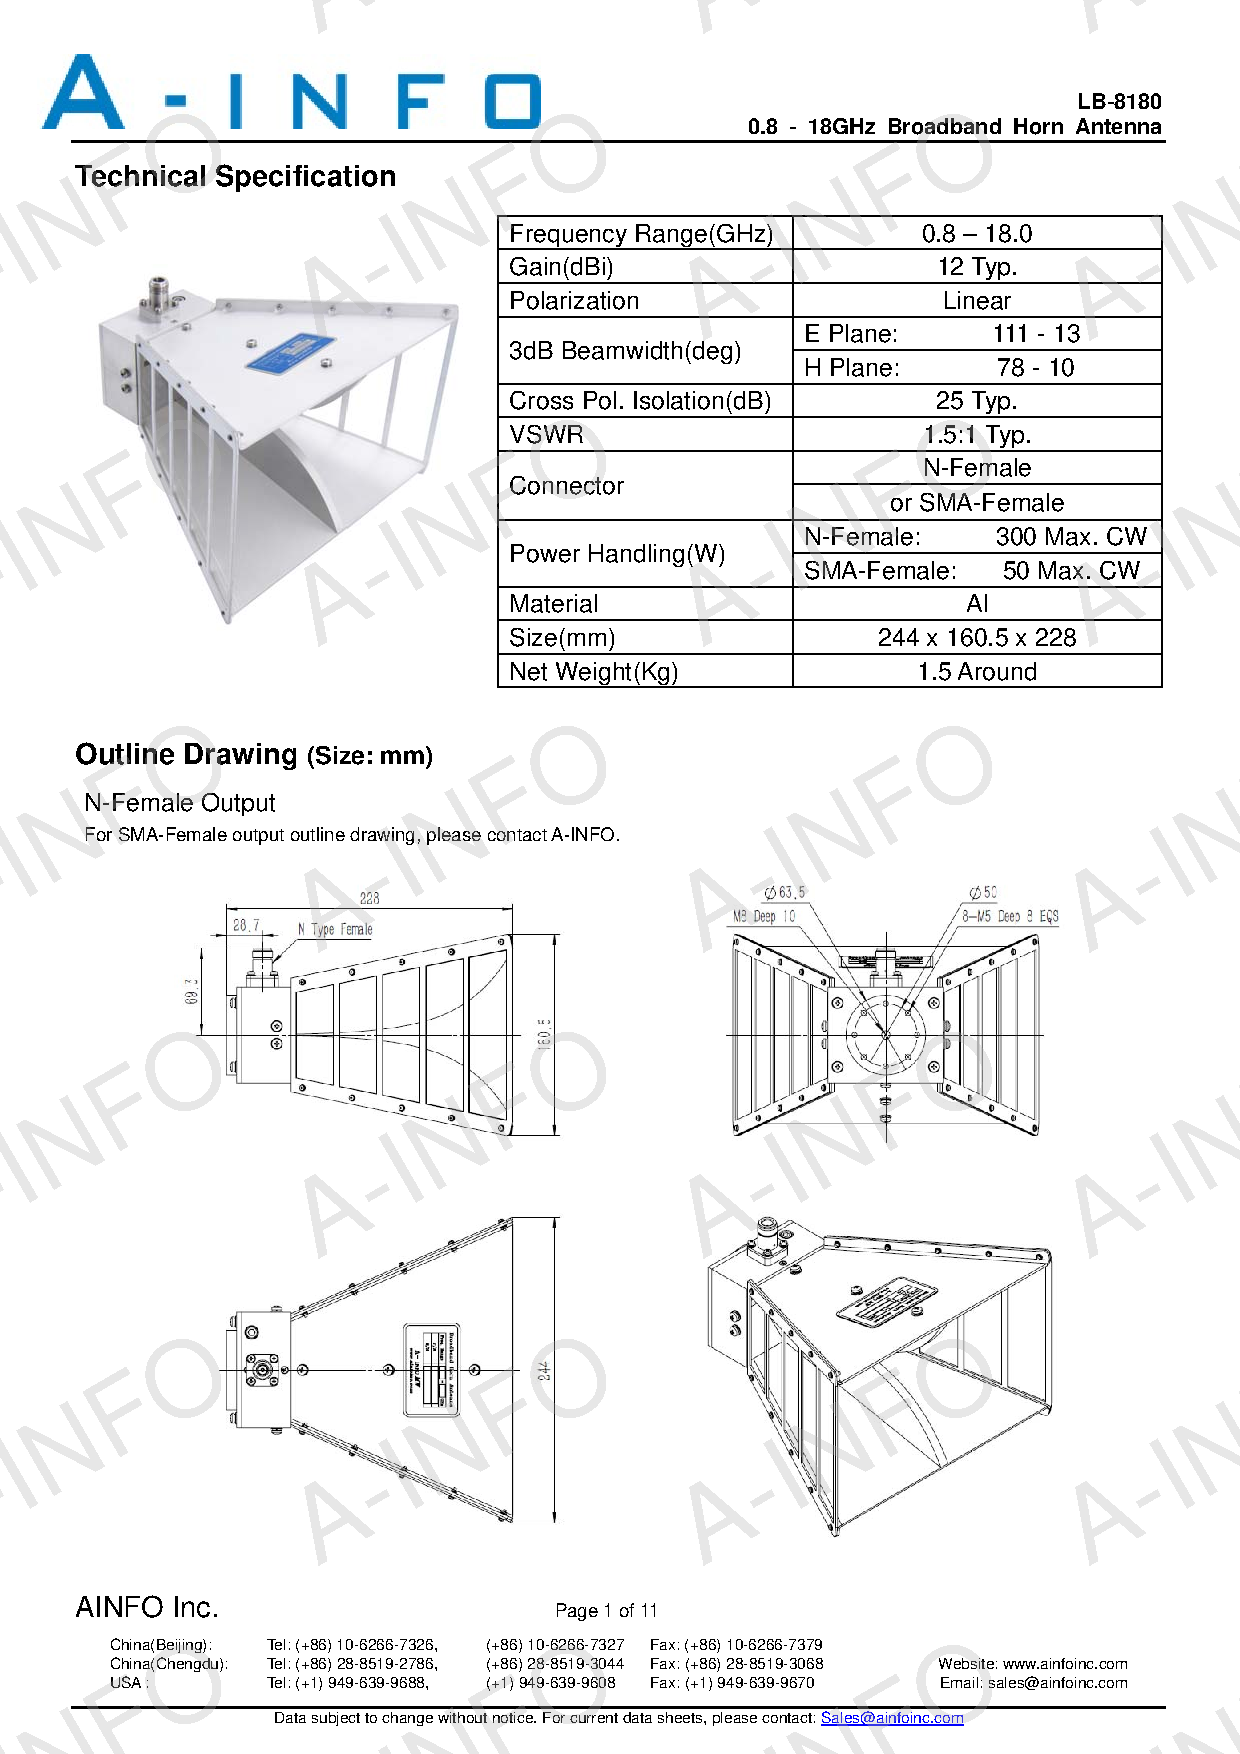
\includepdf[pages = {1}, scale = .75, offset = 0cm -1cm, trim=0.5cm 3cm 1cm 0.5cm, clip, pagecommand=\thispagestyle{empty}\chapter{Datenblatt Hornstrahler (Auszug)}\label{A:Datenblatt_Antennen}]{Anhang/Datenblatt_Antennen.pdf}
\includepdf[pages = {4,5}, scale = .75, offset = 0cm 0cm, trim=0.5cm 3cm 1cm 0.5cm, clip, pagecommand=\thispagestyle{fancy}]{Anhang/Datenblatt_Antennen.pdf}




